\subsection{Matrix matrix multiplication problem}
Matrix matrix multiplication was covered in project 1, and the operation requires $\sim N^3$ floating point operations performed on $\sim N^2$ elements, which means that the problem is compute bound for large matrices. This should be optimal for GPU execution due to the very high number of cores working in parallel. In the following, a GPU program is developed in CUDA 8.0, with incremental steps that would improve the performance.
\subsubsection{GPU1}
The first version is a sequential version only to be run on a single CUDA core. Peroformance wise, this is very uninteresting, but it is a good exercise to ensure that the framework of \texttt{cudaMalloc} and \texttt{cudaMemcpy} is set-up correctly. The code is shown below.

\begin{lstlisting}[caption = gpu1 function with the cuda framework. The kernel \texttt{cudaSeq} is identical to the mkn permutaion from project 1.]
__host__
void matmult_gpu1(int m, int n, int k, double * A, double * B, double * C){

	double *d_A, *d_B, *d_C;
	cudaMalloc(&d_A,n*m*sizeof(double));
	cudaMalloc(&d_B,k*m*sizeof(double));
	cudaMalloc(&d_C,n*k*sizeof(double));

 	cudaMemcpy(d_A,A,n*m*sizeof(double), cudaMemcpyHostToDevice);
 	cudaMemcpy(d_B,B,k*m*sizeof(double), cudaMemcpyHostToDevice);
	
	cudaSeq<<<1,1>>>(m,n,k,d_A,d_B,d_C);
	cudaMemcpy(C,d_C,n*m*sizeof(double), cudaMemcpyDeviceToHost);

	cudaFree(d_A);
	cudaFree(d_B);
	cudaFree(d_C);
}
\end{lstlisting}
The kernel is called with \texttt{<<<1,1>>>} which signifies one block consisting of one thread, and thus the entire operation is done in sequential mode. The kernel is identical to the \texttt{mkn} permutation of project 1, and is not shown here. The framework shown above is identical in all subsequent functions. The performance of \texttt{gpu1} is compared to the DGEMM cblas library function run on 4 threads in figure \ref{fig:gpu1_DGEMM}. In this interval with small matrices the DGEMM routine performs at a quite constant level at around 5-10 GFlops/s, whereas \texttt{gpu1} does about 5 MFlops/s, and thus the performance is different by a factor of 1000. That is expected because a single GPU thread can never realize the parallelization potential of both the problem and the GPU.

\begin{figure}
\centering
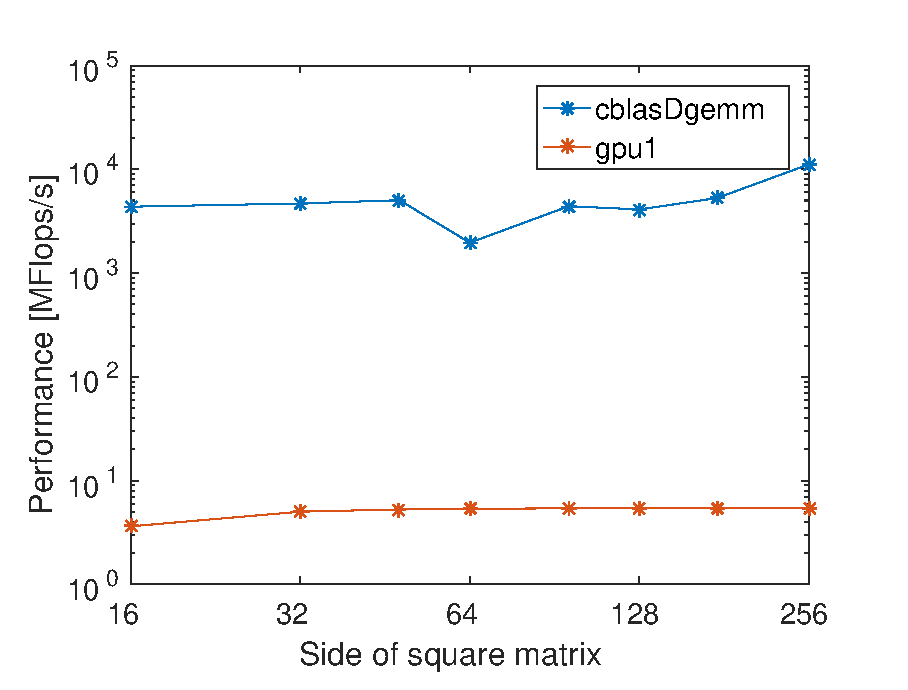
\includegraphics[width = 0.8\textwidth]{fig/gpu1.eps}
\caption{The \texttt{gpu1} function compared to the cblas DGEMM run on 4 cores.}
\label{fig:gpu1_DGEMM}
\end{figure}

\subsubsection{GPU2}
Obviously, using only 1 thread is not the way to use a GPU to increase performance, so in order to better utilize the many threads allowed on a GPU, we now implement a function, \texttt{gpu2}, that uses one thread per element of matrix $C$ is size $m\times n$. The threads are ordered in a 2D grid consisting of \texttt{16$\times$16} threads. The grid size is adapted to the matrix size such that the grid dimension are \texttt{gridx = ceil(n/16)} and \texttt{gridy = ceil(m/16)}. If the matrix size is not a multiple of the block size, excess threads are allocated and not used, but for large matrices, the number of unused threads is small compared to the total number of threads. For small matrices it is thus favourable to have a smaller grid size. The code is shown below.
\begin{lstlisting}[caption = Code sample of the naive implementation with one thread per element in $C$.]
__host__
void matmult_gpu2(int m, int n, int k, double * A, double * B, double * C){	
	int K = 32;
	int gridx = ceil(n*1.0/K);
	int gridy = ceil(m*1.0/K);
	...
	cudaPar<<<dim3(gridx,gridy),dim3(K,K)>>>(m,n,k,d_A,d_B,d_C);
	...
}

__global__
void cudaPar(int m, int n, int k, double * A, double * B, double * C){
	int i = blockIdx.x*blockDim.x + threadIdx.x;
	int j = blockIdx.y*blockDim.y + threadIdx.y;

	if(i < n && j < m){
		C[i + j*n] = 0;

		for(int l = 0; l < k;l++){
			C[j*n + i] += A[k*j + l]*B[l*n + i];
		}
	}
}
	
\end{lstlisting}
The if clause ensures that work is only done inside the matrix, such that none of the excess threads do any unwanted work that could cause a segmentation fault. The last for loop runs through the $k$ elements of A and B in row $j$ and column $i$, and saves the answer sum of the products in the correct element of $C$.

The \texttt{gpu2} function is compared to the cblas DGEMM run on 4 cores for different matrix sizes in figure \ref{fig:gpu2_DGEMM}. For small matrix sizes, the cblasDgemm performs much better than \texttt{gpu2}. This is again due to the limited number of threads being able to operate on a small matrix, simply due to the limited number of elements. As the matrix size increases, the performance increases linearly in this loglog plot, which implies that the behaviour is potential, and most likely quadratic, due to the number of cores increasing with the number of elements, which is $N^2$. At $N \approx 100$ the gpu version performs better, and for $N> 250$, the performance of \texttt{gpu2} flattens out, to stabilize at $\sim 55$ GFlops/s, which is around 2.5 times more than the cblasDgemm, which tops at $\sim 22$ GFlops/s. The flattening of the performance of \texttt{gpu2} is analysed with the Nvidia profiler. The results  for square matrices of size 1024 show that L2 cache bandwidth is only used at $\sim 50 \%$. Since the problem is compute bound, the way to improve performance is to increase the cache usage, and make use of the much higher bandwidth from cache to processor than from global memory to processor. When the cache memory is utilized satisfactorily, the memory usage from the global memory to the caches should be optimized. The matrix multiplication takes about 120 ms to run.

\begin{figure}
\centering
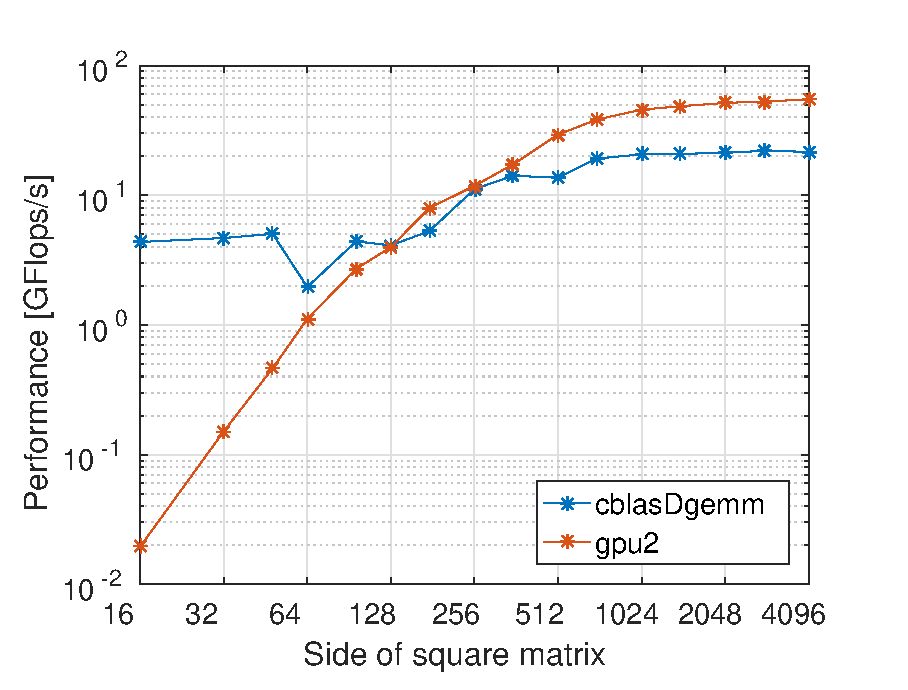
\includegraphics[width = 0.8\textwidth]{fig/gpu2.eps}
\caption{Performance of the \texttt{gpu2} function and the cblas DGEMM for different matrix sizes.}
\label{fig:gpu2_DGEMM}
\end{figure}

\subsubsection{GPU3}
As an attempt to improve memory usage form the caches the gpu function, we now changed \texttt{gpu2} to use half as many threads, but have each thread update 2 adjacent values of the $C$ matrix. We choose to have each thread do its own element and the one below. This choice is made to ensure coalesced memory reads in matrix A, which is used row wise by each thread, and a single cache line of 128 bytes thus fits with the warp size of 32 threads. Matrix B is still read in a non-coalesced manner, but that will be the case no matter which neighbour is chosen. For larger matrices, decreasing the number of threads has no immediate effect on the performance due to the fact that the matrix multiplication of large matrices is a compute bound operation, the limiting factor is the available CUDA cores that can perform flops in parallel, but since we cannot change that we chose to improve the cache usage. The $y$-dimension of the grid is now \texttt{gridy = ceil(m/16/2)}, but otherwise the framework is the same. The kernel source code is seen below. The inner loop is over $p$ to increase the memory re-usage of the $B$ matrix, and it has been written out explicitly to get rid of the overhead. The first if clause takes care of the threads that can do both elements, and the second if clause take the threads which cannot compute both elements assigned to it due to the last one being out of bounds.

\begin{lstlisting}[caption = The source code for texttt{gpu3}. The $l$ loop is the outer loop to increase memory re-usage.]
__global__
void cudaPar2(int m, int n, int k, int p, double * A, double * B, double * C){
	const int P = 2;
	double C_r[P]={0.0,0.0};

	int i = blockIdx.x*blockDim.x + threadIdx.x;
	int j = blockIdx.y*blockDim.y + threadIdx.y;

	j = j*p; // allows C[i + (0/1) j*n] indexing
	if(i < n && j < m-p + 1){
		for(int l = 0; l < k; l++){
			C_r[0] += A[(j + 0)*k + l]*B[n*l + i];
			C_r[1] += A[(j + 1)*k + l]*B[n*l + i];
		}
		for(int pp = 0; pp < p; pp++) C[(j + pp)*n + i] =  C_r[pp];
	}
	if(i < n && j > m-p && j < m){
		for(int l = 0; l < k; l++){
			C_r[0] += A[(j + 0)*k + l]*B[n*l + i];
			C_r[1] += A[(j + 1)*k + l]*B[n*l + i];
		}
		for(int pp = 0; pp < p; pp++) C[(j + pp)*n + i] =  C_r[pp];
	}
}
\end{lstlisting}
The performance of \texttt{gpu3} is compared to the \texttt{gpu2} and \texttt{cblasDgemm} is figure \ref{fig:gpu3}, and we see that \texttt{gpu3} performs better for $N > 100$, and increases to perform twice as well for a matrix size of 4096 with $\sim 100$ GFLops/s. For a similar case analysed with \texttt{gpu2}, square matrices of size 1024 are investigated with \texttt{gpu3}. We have a 50 \% increase in the usage of the L2 cache bandwidth and the global memory bandwidth, and as a result, the run time for each call is down by 17 \% to about 100 ms.

\begin{figure}
\centering
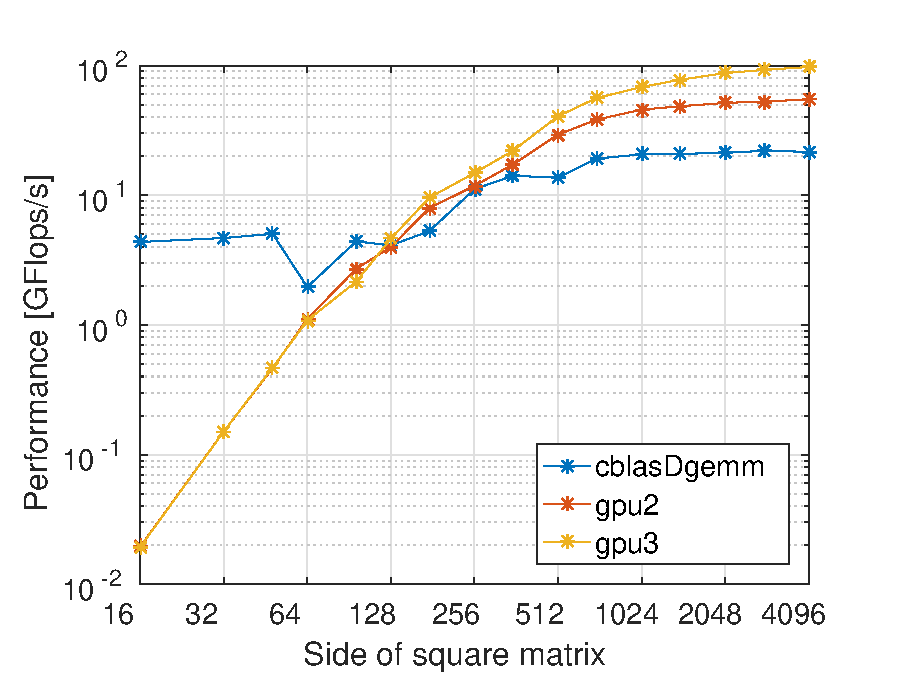
\includegraphics[width = 0.8\textwidth]{fig/gpu3.eps}
\caption{Performance of \texttt{gpu2}, \texttt{gpu3} and the cblasDgemm functions for increasing matrix sizes.}
\label{fig:gpu3}
\end{figure}
\subsubsection{GPU4}
In an attempt to increase the reuse of the column of $B$ each thread loads, we increased $p$ to 4. For large matrices, there are still threads enough to have threads calculation on the CUDA cores, and the memory that is required to be loaded from the global memory is significantly reduced, which even though it is a compute bound problem, should increase the performance, due to better cache utilization. The source code for \texttt{gpu4} is much alike that of \texttt{gpu3}, but for completeness, it is included below.
\begin{lstlisting}[caption = The source code for texttt{gpu4}. The $l$ loop is the outer loop to increase memory re-usage.]
__global__
void cudaPar4(int m, int n, int k, int p, double * A, double * B, double * C){
	const int P = 4;
	double C_r[P]={0.0,0.0,0.0,0.0};

	int i = blockIdx.x*blockDim.x + threadIdx.x;
	int j = blockIdx.y*blockDim.y + threadIdx.y;

	j = j*p; // allows C[i + (0/1) j*n] indexing
	if(i < n && j < m-p + 1){
		for(int l = 0; l < k; l++){
			C_r[0] += A[(j + 0)*k + l]*B[n*l + i];
			C_r[1] += A[(j + 1)*k + l]*B[n*l + i];
			C_r[2] += A[(j + 2)*k + l]*B[n*l + i];
			C_r[3] += A[(j + 3)*k + l]*B[n*l + i];
		}
		for(int pp = 0; pp < p; pp++) C[(j + pp)*n + i] =  C_r[pp];
	}
	if(i < n && j > m-p && j < m){
		for(int l = 0; l < k; l++){
			C_r[0] += A[(j + 0)*k + l]*B[n*l + i];
			C_r[1] += A[(j + 1)*k + l]*B[n*l + i];
			C_r[2] += A[(j + 2)*k + l]*B[n*l + i];
			C_r[3] += A[(j + 3)*k + l]*B[n*l + i];
		}
		for(int pp = 0; pp < p; pp++) C[(j + pp)*n + i] =  C_r[pp];
	}
}
\end{lstlisting}
The performance of \texttt{gpu4} is compared to the previous functions in figure \ref{fig:gpu4}, and we observe a slight increase in performance to about 108 GFlops/s, but much the same behaviour as expected due to the similarity of the code. The profiler shows that the used bandwidth in both L2 cache and global memory is increased by $\sim 10 \%$. The increase of $p$ from two to four, only gave a 10 \% increase, so increasing p further is not likely to be worthwhile.

\begin{figure}
\centering
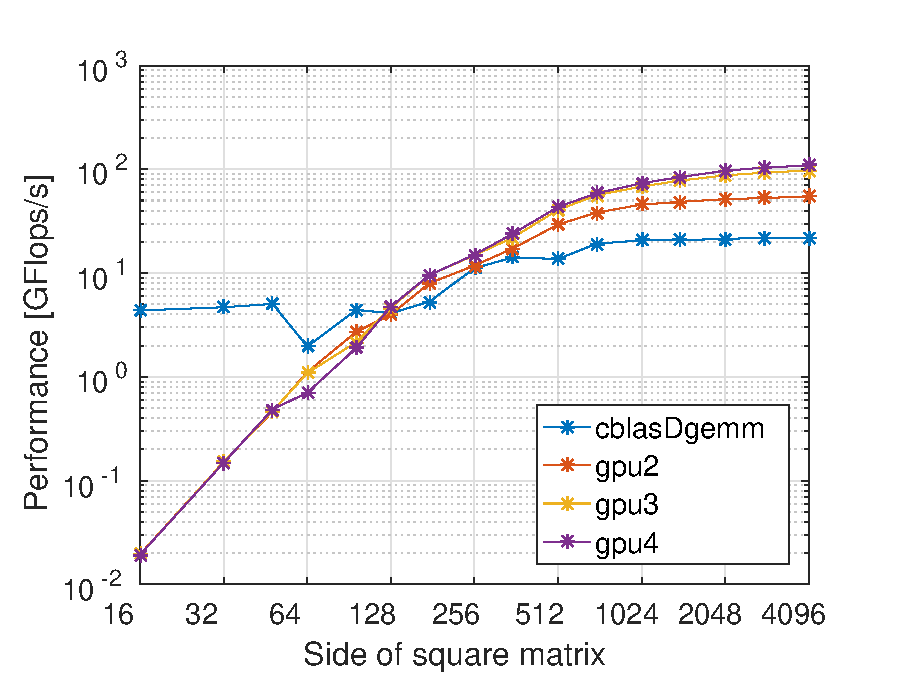
\includegraphics[width = 0.8\textwidth]{fig/gpu4.eps}
\caption{Performance of the gpu functions and the cblasDgemm as a function of matrix size.}
\label{fig:gpu4}
\end{figure}


\subsubsection{GPU5}
Instead, we now attempt to utilize the shared memory each block has. The bottleneck is now likely the non-coalesced reads from the $B$ matrix, and so by utilising the shared memory one can read blocks of both matrices in a coalesced manner, store the loaded blocks in shared memory and do the multiplication on the blocks, store the result in a third shared memory variable, and then move the blocks along $A$ and $B$, and at the end, the last shared memory variable can be saved to $C$. In this way, the L1 cache bandwidth is now utilised properly. The approach is similar to the blocking exercise in project 1, only here the memory management is done explicitly. The source code is shown below.

\begin{lstlisting}[caption = Source code for the shared memory kernel]
__global__
void cudaSMEM(int m, int n, int k, double * A, double * B, double * C){
	const int K = 32;	
	int kk = k/K;

	int i = blockIdx.x*blockDim.x + threadIdx.x;
	int j = blockIdx.y*blockDim.y + threadIdx.y;
	int iBlock = threadIdx.x;
	int jBlock = threadIdx.y;


	__shared__ double smemA[K][K];
	__shared__ double smemB[K][K];
	__shared__ double smemC[K][K];

	smemC[jBlock][iBlock] = 0;

	for(int q = 0; q < kk; q++){
		smemB[jBlock][iBlock] = B[i + q*K*n + jBlock*n];
		smemA[jBlock][iBlock] = A[iBlock + j*k + q*K];
		__syncthreads();
		for(int z = 0; z < K; z++){
			smemC[jBlock][iBlock] += smemA[jBlock][z]*smemB[z][iBlock];
		}
		__syncthreads();
	}
	C[i + j*n] = smemC[jBlock][iBlock];
}
\end{lstlisting}
In this case, a block size of 32 is used. This choice means that each warp now make up a single row in each block, and the cache lines consist of 32 floats, which means that each warp requires only 1 cache line per block, which optimizes the memory transfers. Each threads block does a matrix-block of the same size, so each thread does one element of $C$. Three 32 by 32 blocks is about 25 MB, so a block size of 64 will not fit in the shared memory which is 49 MB. Block sizes of non-multiples of 32 will cause unused data to be loaded, taking up bandwidth which is of course not desirable.

The performance of \texttt{gpu5} is added to the plot, and it is seen in figure \ref{fig:gpu5}. For large matrices of size $N>2000$, the performance is about 200 GFlops/s, which is about twice as good as \texttt{gpu4}.Unfortunately, \texttt{gpu5} does not perform well on cuda 6.5, which is used for the analyser, so that can not back up the claims, but a factor of 2 speed up is a great result.

\begin{figure}
\centering
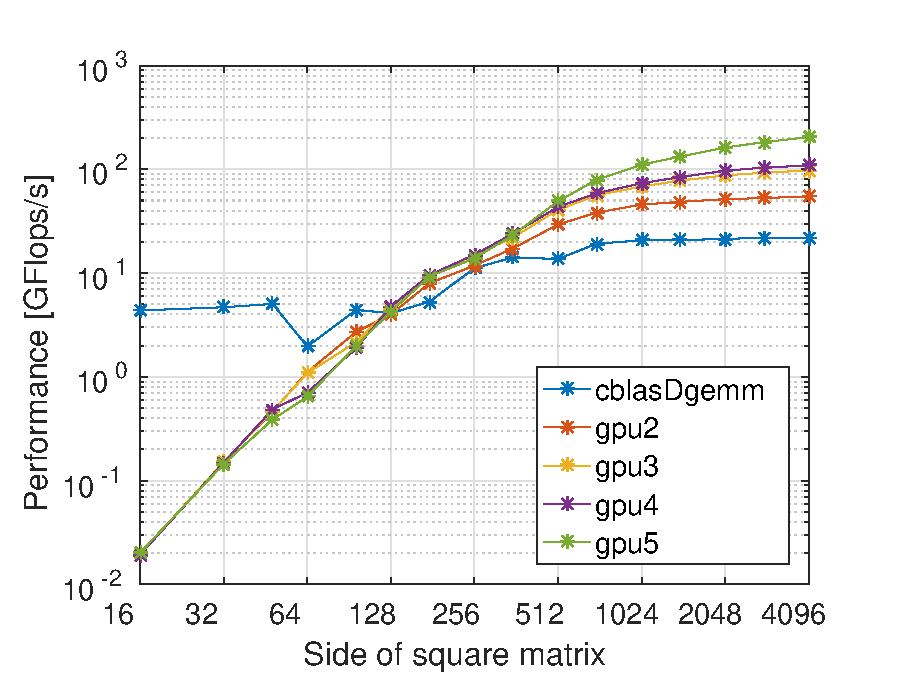
\includegraphics[width = 0.8\textwidth]{fig/gpu5.eps}
\caption{Performance of the gpu functions and the cblasDgemm library function. \texttt{gpu5} is seen to be roughly a factor of 2 faster than \texttt{gpu4}.}
\label{fig:gpu5}
\end{figure}
Compared to the theoretical maximum of $745$ MHz $\times 2880 \approx 2 THz$, we only utilize 10 \% of the clock cycles, but as evident form figure \ref{fig:gpu5}, the \texttt{gpu5} curve is still increasing at $N =4000$, so a higher fraction could be possible with larger matrices. The optimization is of course not finished with this, but no more optimizations are carried out. Further changes could be to split up $C$ into smaller parts, to make use of the fact that the elements of $C$ are independent, and thereby the problem allows for asynchronous memory copying. This could hide the latency, which for \texttt{gpu5} takes $\sim 10\%$ of the gpu time. Since the problem is compute bound, an obvious improvement would be to split up the matrix and compute each half on two different GPUs as it is done in the Poisson exercise. That would double the number of available CUDA cores, which should do great in bringing the wall time down, but in turn would not improve the resource utilization.

\subsubsection{GPULIB}
Finally, Nvidia has created a BLAS version called cublas optimized for the GPU, and as we implemented it as \texttt{gpulib}. The \texttt{cublasDgemm} takes the matrices as column major, so with the row major form of C, care must be taken to ensure a correct result. First, we realize that a row major matrix read as column major is the transposed matrix, i.e.
\begin{equation}
A_C = A_R^T,
\end{equation}
where superscript T denotes transpose, and subscript R/C denotes whether the matrix is read column wise or row wise. We assume that all matrices are stored row wise. We then realize that if $C_R = A_R\times B_R$, then $C_R^T = B_R^T \times A_R^T = B_C \times A_C = C_C$. So by $B$ and $A$ to cublasDgemm, the result $C_C = C_R^T$ is the transposed of what we are after. This, however, fixes itself, as C reads the matrix in row major format, effectively performing a transpose: $C_C^T = (C_R^T)^T = C_R$ which is the desired result.

The cublasDgemm routine is applied to the same matrix sizes used for the other functions, and the comparison can be seen in figure \ref{fig:gpuALL}. The performance of the cublas function continues to increase at $N =4096$, but there the performance is already 540 Gflops/s, which is about a quarter of the theoretical maximum. It is worth noting, that the cublas functions is the poorest of all for small matrices, highlighting the fact that it is optimizes to large matrices. However, for small matrices with a side length of $N< 100$, one should never attempt to go to the GPU.

\begin{figure}
\centering
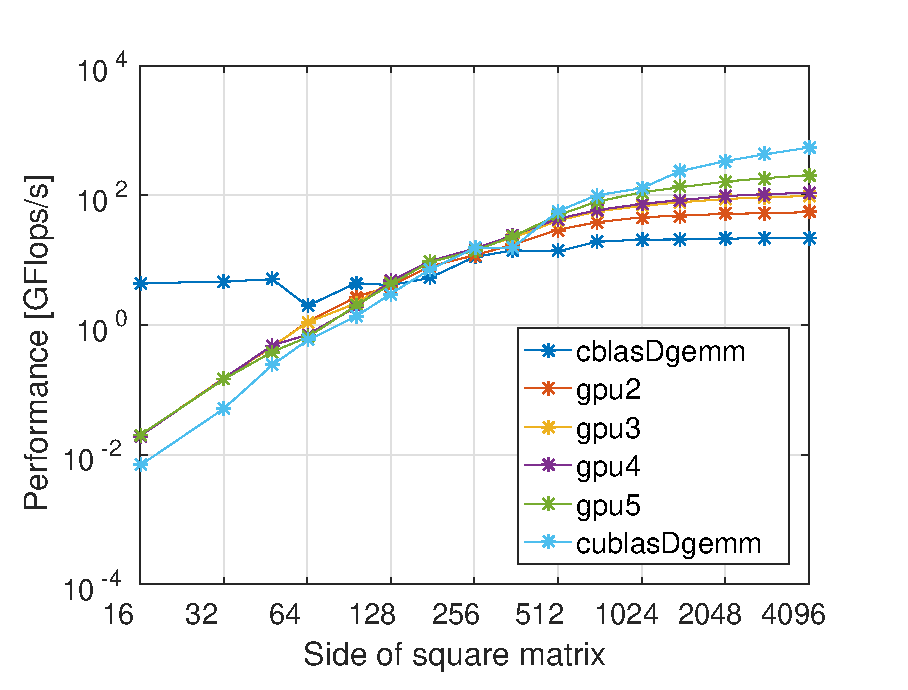
\includegraphics[width = 0.8\textwidth]{fig/gpulib.eps}
\caption{Performance of gpu2 to gpu5, the cublas function, and the cblas function versus the matrix size.}
\label{fig:gpuALL}
\end{figure}